\chapter{Direct estimation}

In this chapter the steps of developing the chosen AI models for estimating vehicle speeds will be discussed. First, the simple recurrent neural network (RNN) will be presented. This will be followed by two more specific RNN models: long short-term memory (LSTM) and gated recurrent unit (GRU). All of these models will be trained and tuned to directly estimate the longitudinal and lateral speeds of the vehicle from the previously discussed CAN signals.

\section{Recurrent Neural Network - RNN}

\subsection{Theoretical background}

Contrary with regular feedforward neural networks where the output is determined only by the current values of the inputs, the RNN is designed in a way that after each step the information is fed back to the network. This way the output will be dependent on the previous inputs as well and the model will have a memory like property giving the possibility of handling temporal data.

\FloatBarrier
\begin{figure}[h]
    \centering
    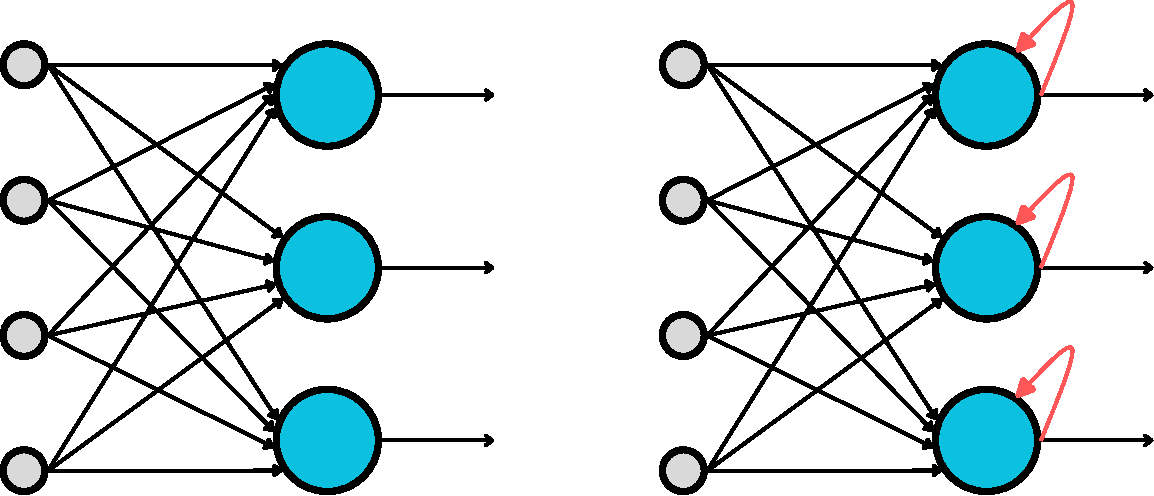
\includegraphics[width=0.8\textwidth]{images/feedforward vs recurrent.pdf}
    \caption{Feedforward nn (left) compared to recurrent nn (right)}
    \label{fig:NNvsRNN}
\end{figure}
\FloatBarrier

The fundamental building blocks of a RNN are the recurrent units (RU). These units hold an inner state that connect the in- and outputs. The inner states maintain information about previous inputs in a sequence. To understand how does the network's architecture function, let it be unfolded in time. This can be seen on figure \ref{fig:unfolded_RNN}.

\FloatBarrier
\begin{figure}[h]
    \centering
    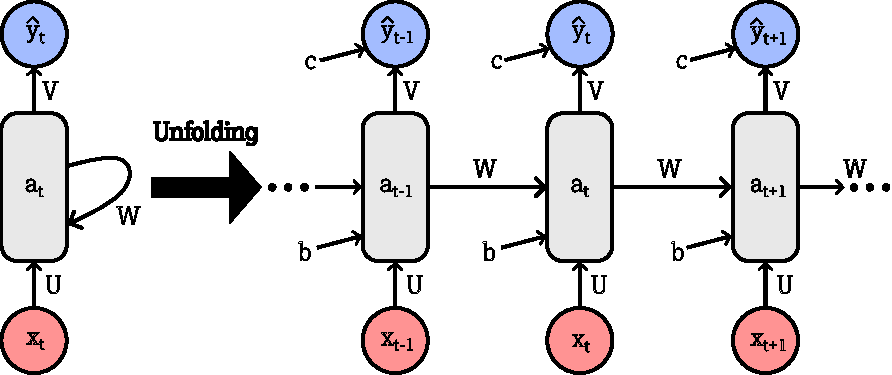
\includegraphics[width=0.8\textwidth]{images/unfolded_rnn.pdf}
    \caption{Unfolding the architecture of a RNN in time}
    \label{fig:unfolded_RNN}
\end{figure}
\FloatBarrier

It is visible that at time step $t$ the output vector ($\hat y_t$) is determined by the state of the hidden layer ($a_t$). However the hidden layer is determined by the previous state of the hidden layer ($a_{t-1}$) and the input vector ($x_t$) of the current timestep $t$, that can be written as
\begin{equation}
    a_t = f(a_{t-1}, x_t; \theta),
\end{equation}
where $\theta$ represents the biases ($b$) and weights ($U, W$)  and $f()$ is the activation function (e.g tanh()). This equation can be expanded as
\begin{equation}
    a_t = f(U\cdot x_t + W \cdot a_{t-1} + b),
\end{equation}
where $U$ is the weight matrix connecting the input layer and the hidden layer, $W$ is the weight matrix to connect the hidden layer's previous state and the current state and $b$ is the bias vector for the hidden layer. From this the output vector can be determined as
\begin{equation}
    \hat y_t = g(V \cdot a_t + c),
\end{equation}
where $V$ is the weight matrix connecting the hidden layer and the output vector, $c$ is the bias vector for the output layer and $g()$ is the activation function (e.g softmax()).

To determine the weights and biases of the network backpropagation through time (BPTT) is used, that is an extended version of the backpropagation used in FNNs. This method is based on the error between the determined output of the network and the desired/labeled output at time step $t$. BPTT involves two major steps: forward pass and backward pass. These steps are detailed below:

\begin{enumerate}
    \item Forward pass
    \begin{itemize}
        \item During the forward pass the sequence of inputs form $t=1$ to $t=n$ passes through the network, where $n$ is the length of the sequence.
        \item The output vector $y_t$ is determined at every timestep with the use of the previously described formulas. 
        \item The loss is calculated at every timestep between the desired ($y_t$) and the calculated ($\hat y_t$) output. 
        \item The loss function is given by the mean squared error (MSELoss):
        \begin{equation}
            L(y, \hat y) = \frac{1}{t} \sum_{t=1}^{n} (y_t - \hat y_t)^2
        \end{equation}
    \end{itemize}
    \item Backward pass
        \begin{itemize}
        \item During the backward pass the gradients of the loss function  $L(y, \hat y)$ are calculated with respect of the weights of the network ($U, V, W$). 
        \item W.r.t the weight matrices the derivatives of the loss functions can be determined as:
        \begin{equation}
            \frac{\partial L}{\partial U} = \sum_{t=1}^n \frac{\partial L}{\partial a_t} \cdot \frac{\partial a_t}{\partial U}
        \end{equation}
        \begin{equation}
            \frac{\partial L}{\partial W} = \sum_{t=1}^n \frac{\partial L}{\partial a_t} \cdot \frac{\partial a_t}{\partial W}
        \end{equation}
        \begin{equation}
            \frac{\partial L}{\partial V} = \sum_{t=1}^n \frac{\partial L}{\partial \hat y_t} \cdot \frac{\partial \hat y_t}{\partial V}
        \end{equation}
        \item The gradient values inform about the direction (increase or decrease) and the magnitude of the change in the weight matrices. 
        \item These gradients can then be used for updating the values of each weight matrix with the help of the chosen optimizer (e.g. SGD, Adam).
    \end{itemize}
\end{enumerate}

Common issues when applying RNNs are exploding and vanishing gradients during the backward pass. Both of these refer to the magnitude of the calculated gradients: $\left\Vert \frac{\partial L}{\partial W} \right\Vert$. Exploding gradient problem stems from the gradient being too high which is a consequence of the learning rate being to big. On the other hand vanishing gradient refers to a gradient being near zero, which leads to slow learning. 

\subsection{Implementing a RNN}

When implementing a RNN architecture for a specific application, there are some general hyperparameters to determine. These parameters can be found in table \ref{tab:rnn_hyperparams}.

\begin{table}[h]
\centering
\resizebox{\textwidth}{!}{%
\begin{tabular}{@{}ll@{}}
\toprule
\textbf{Hyperparameter}     & \textbf{Description} \\ 
\midrule
\emph{Model Architecture:} & \\ 
Hidden size                & Dimensionality of the hidden (and cell) state vector at each time step. \\
Number of layers           & Number of stacked RNN/LSTM/GRU layers (depth of the model). \\
Cell type                  & RNN variant (vanilla RNN, LSTM, GRU). \\
Bidirectionality           & Whether to process the sequence in both forward and backward directions. \\
Dropout rate               & Fraction of units dropped between layers to prevent overfitting. \\[\smallskipamount]
\midrule
\emph{Training Configuration:} & \\ 
Learning rate              & Step size for weight updates in gradient descent. \\
Optimizer                  & Algorithm for updating parameters (SGD, Adam, RMSProp, etc.). \\
Batch size                 & Number of sequences processed per gradient update. \\
Number of epochs           & Full passes over the training dataset. \\
Gradient clipping          & Maximum norm for gradients to prevent exploding gradients. \\
Sequence length            & Number of time steps in each input subsequence (truncated BPTT window). \\[\smallskipamount]
\midrule
\emph{Regularization:} & \\ 
Weight decay               & L2 penalty on weights to discourage large values. \\
Early stopping             & Halt training if validation loss stops improving. \\[\smallskipamount]
\midrule
\emph{Data‐related:} & \\ 
Normalization method       & How inputs are scaled (min–max, z‑score, etc.). \\
Input window size          & How many past time steps are fed to the network. \\
Prediction horizon         & How many future steps the network is trained to predict. \\
\bottomrule
\end{tabular}%
}
\caption{Key hyperparameters for RNN‐based sequence models}
\label{tab:rnn_hyperparams}
\end{table}

\subsection{Results}

The used data that was created from 4 simulations that covered 4 basic driving situations. These are: accelerate until a certain longitudinal acceleration (auax-drv), brake until a certain longitudinal acceleration (buax-brk), steer until a certain lateral acceleration (suay) and sine wave like steering (sin-steer). This way a range of driving situations can be covered. To create more datasets, random values were used within a certain range for the same simulations types. 

The results can be seen on figures below.
\FloatBarrier
\begin{figure}[htbp]
    \centering

    % Second row
    \begin{subfigure}{1\textwidth}
        \centering
        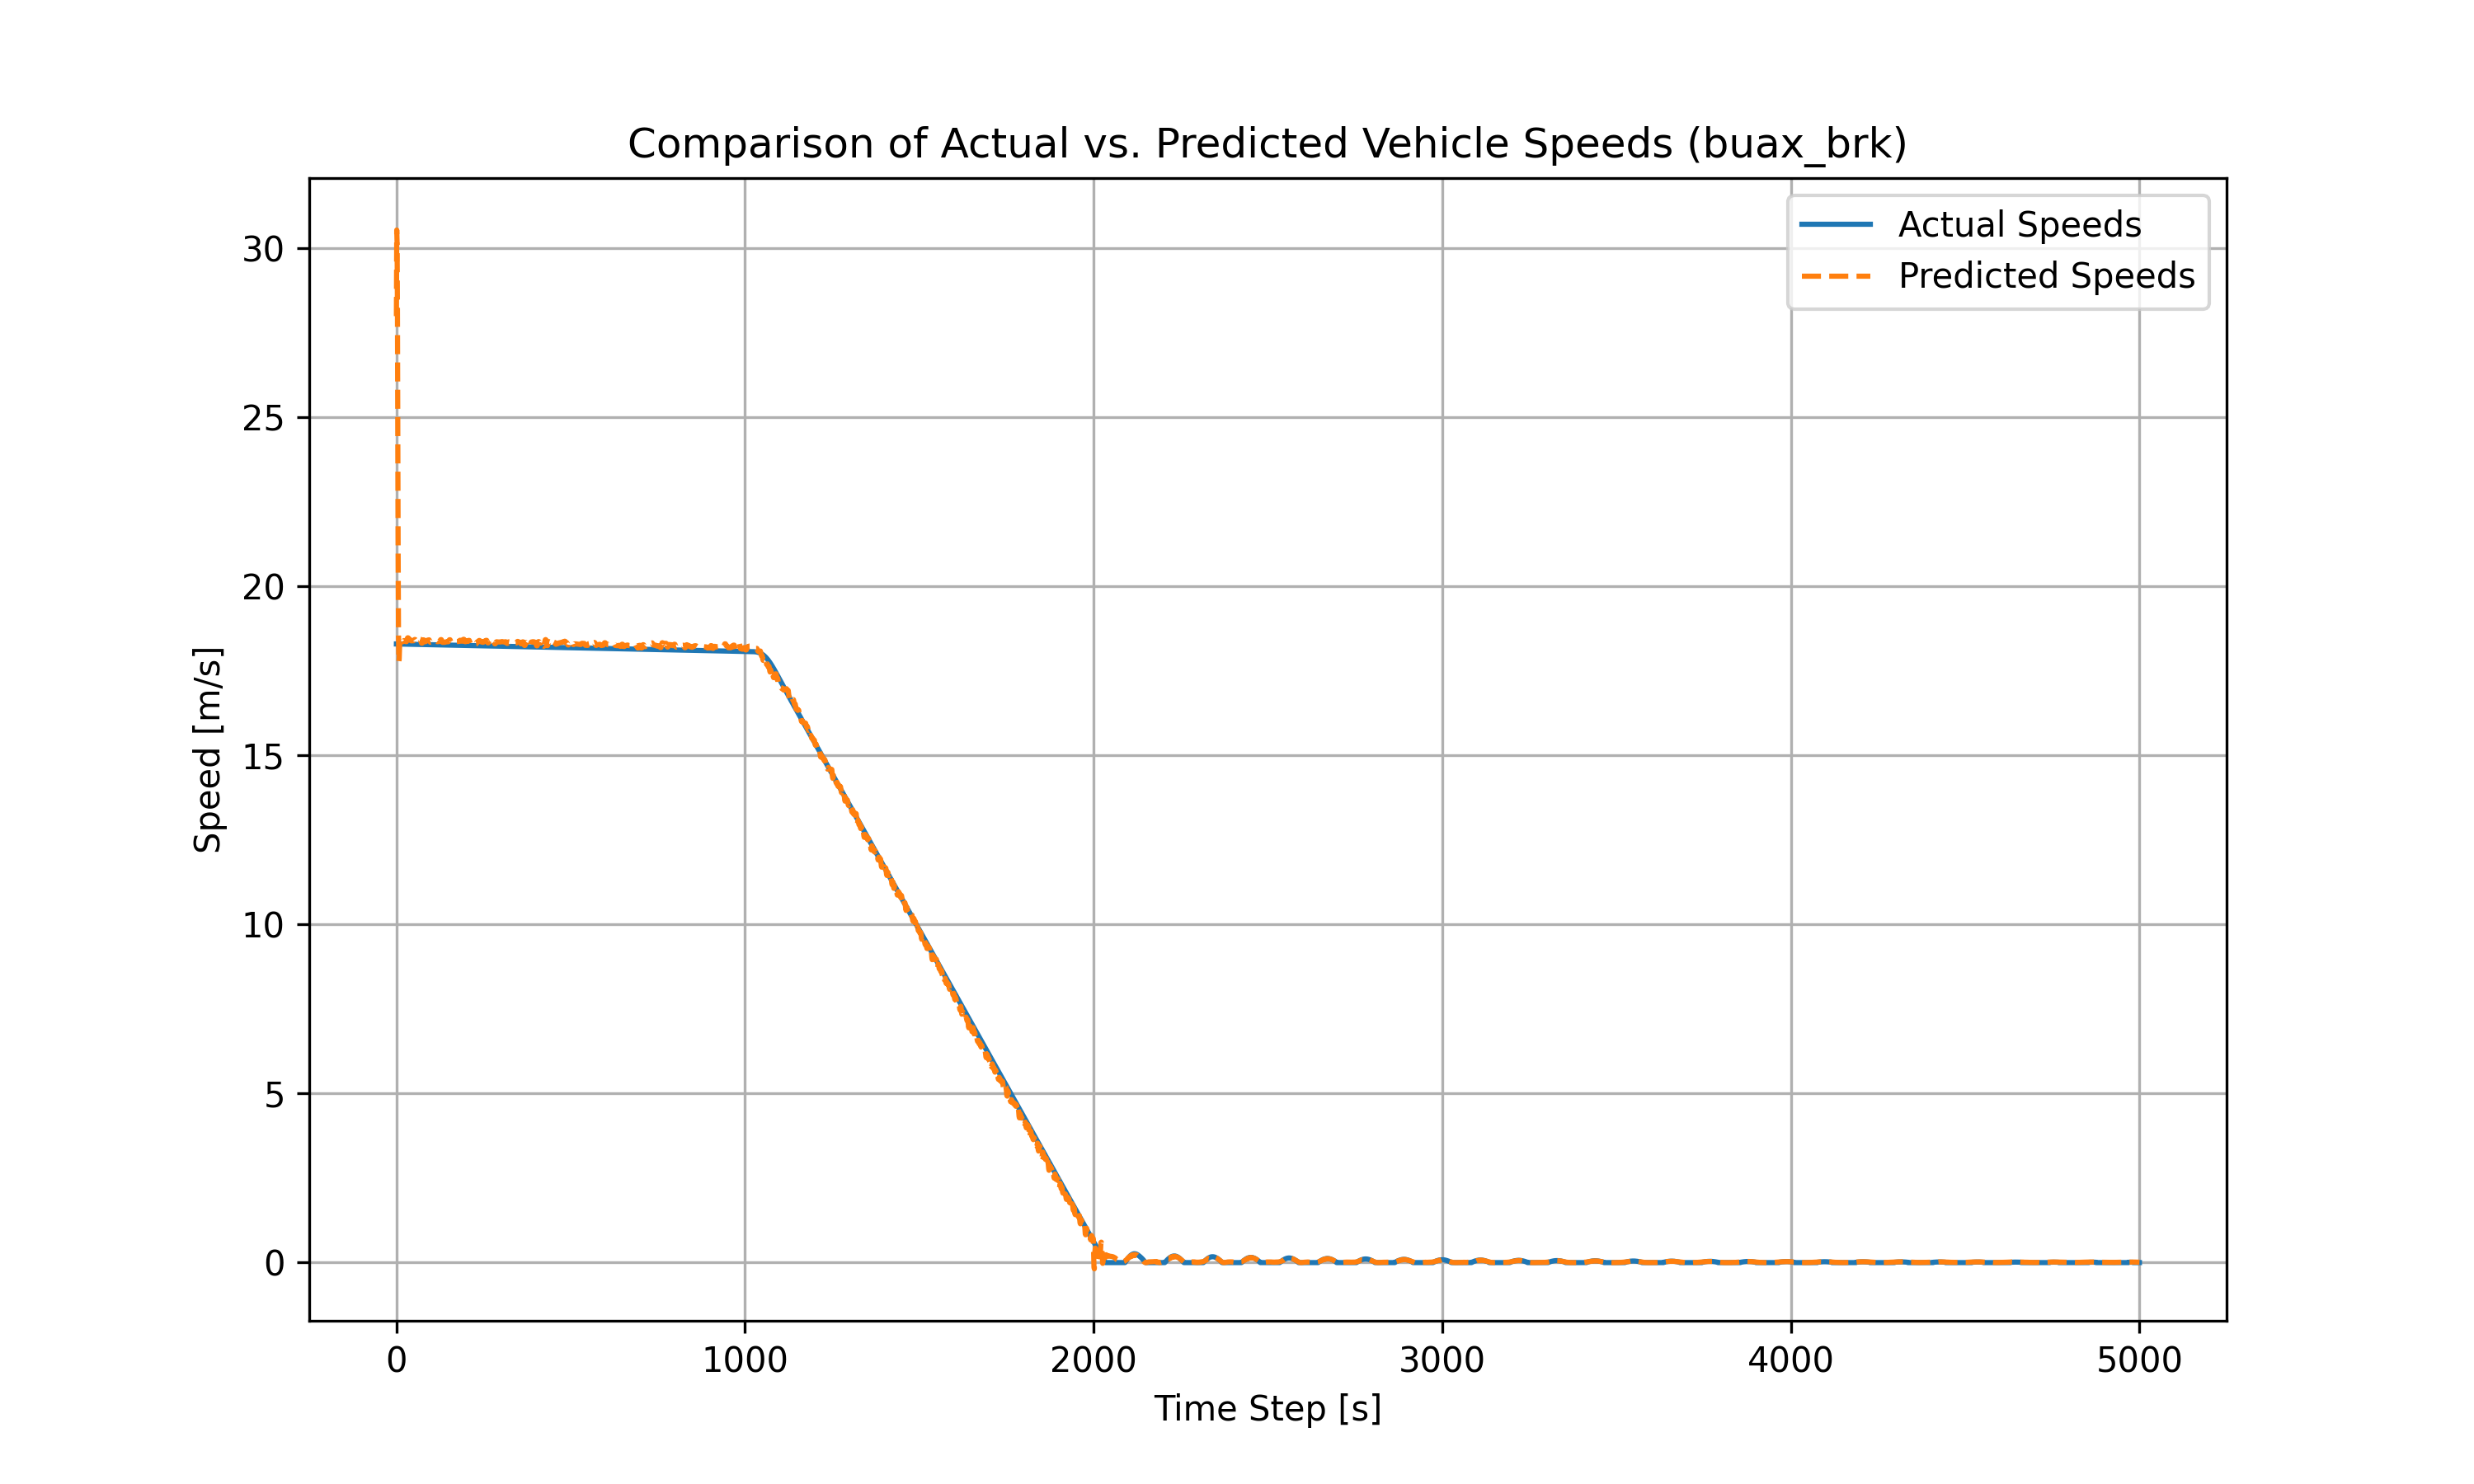
\includegraphics[width=\linewidth]{images/RNN_results/model_0_buax_brk_act_vs_predicted_speed.png}
    \end{subfigure}
    \hfill
    \begin{subfigure}{1\textwidth}
        \centering
        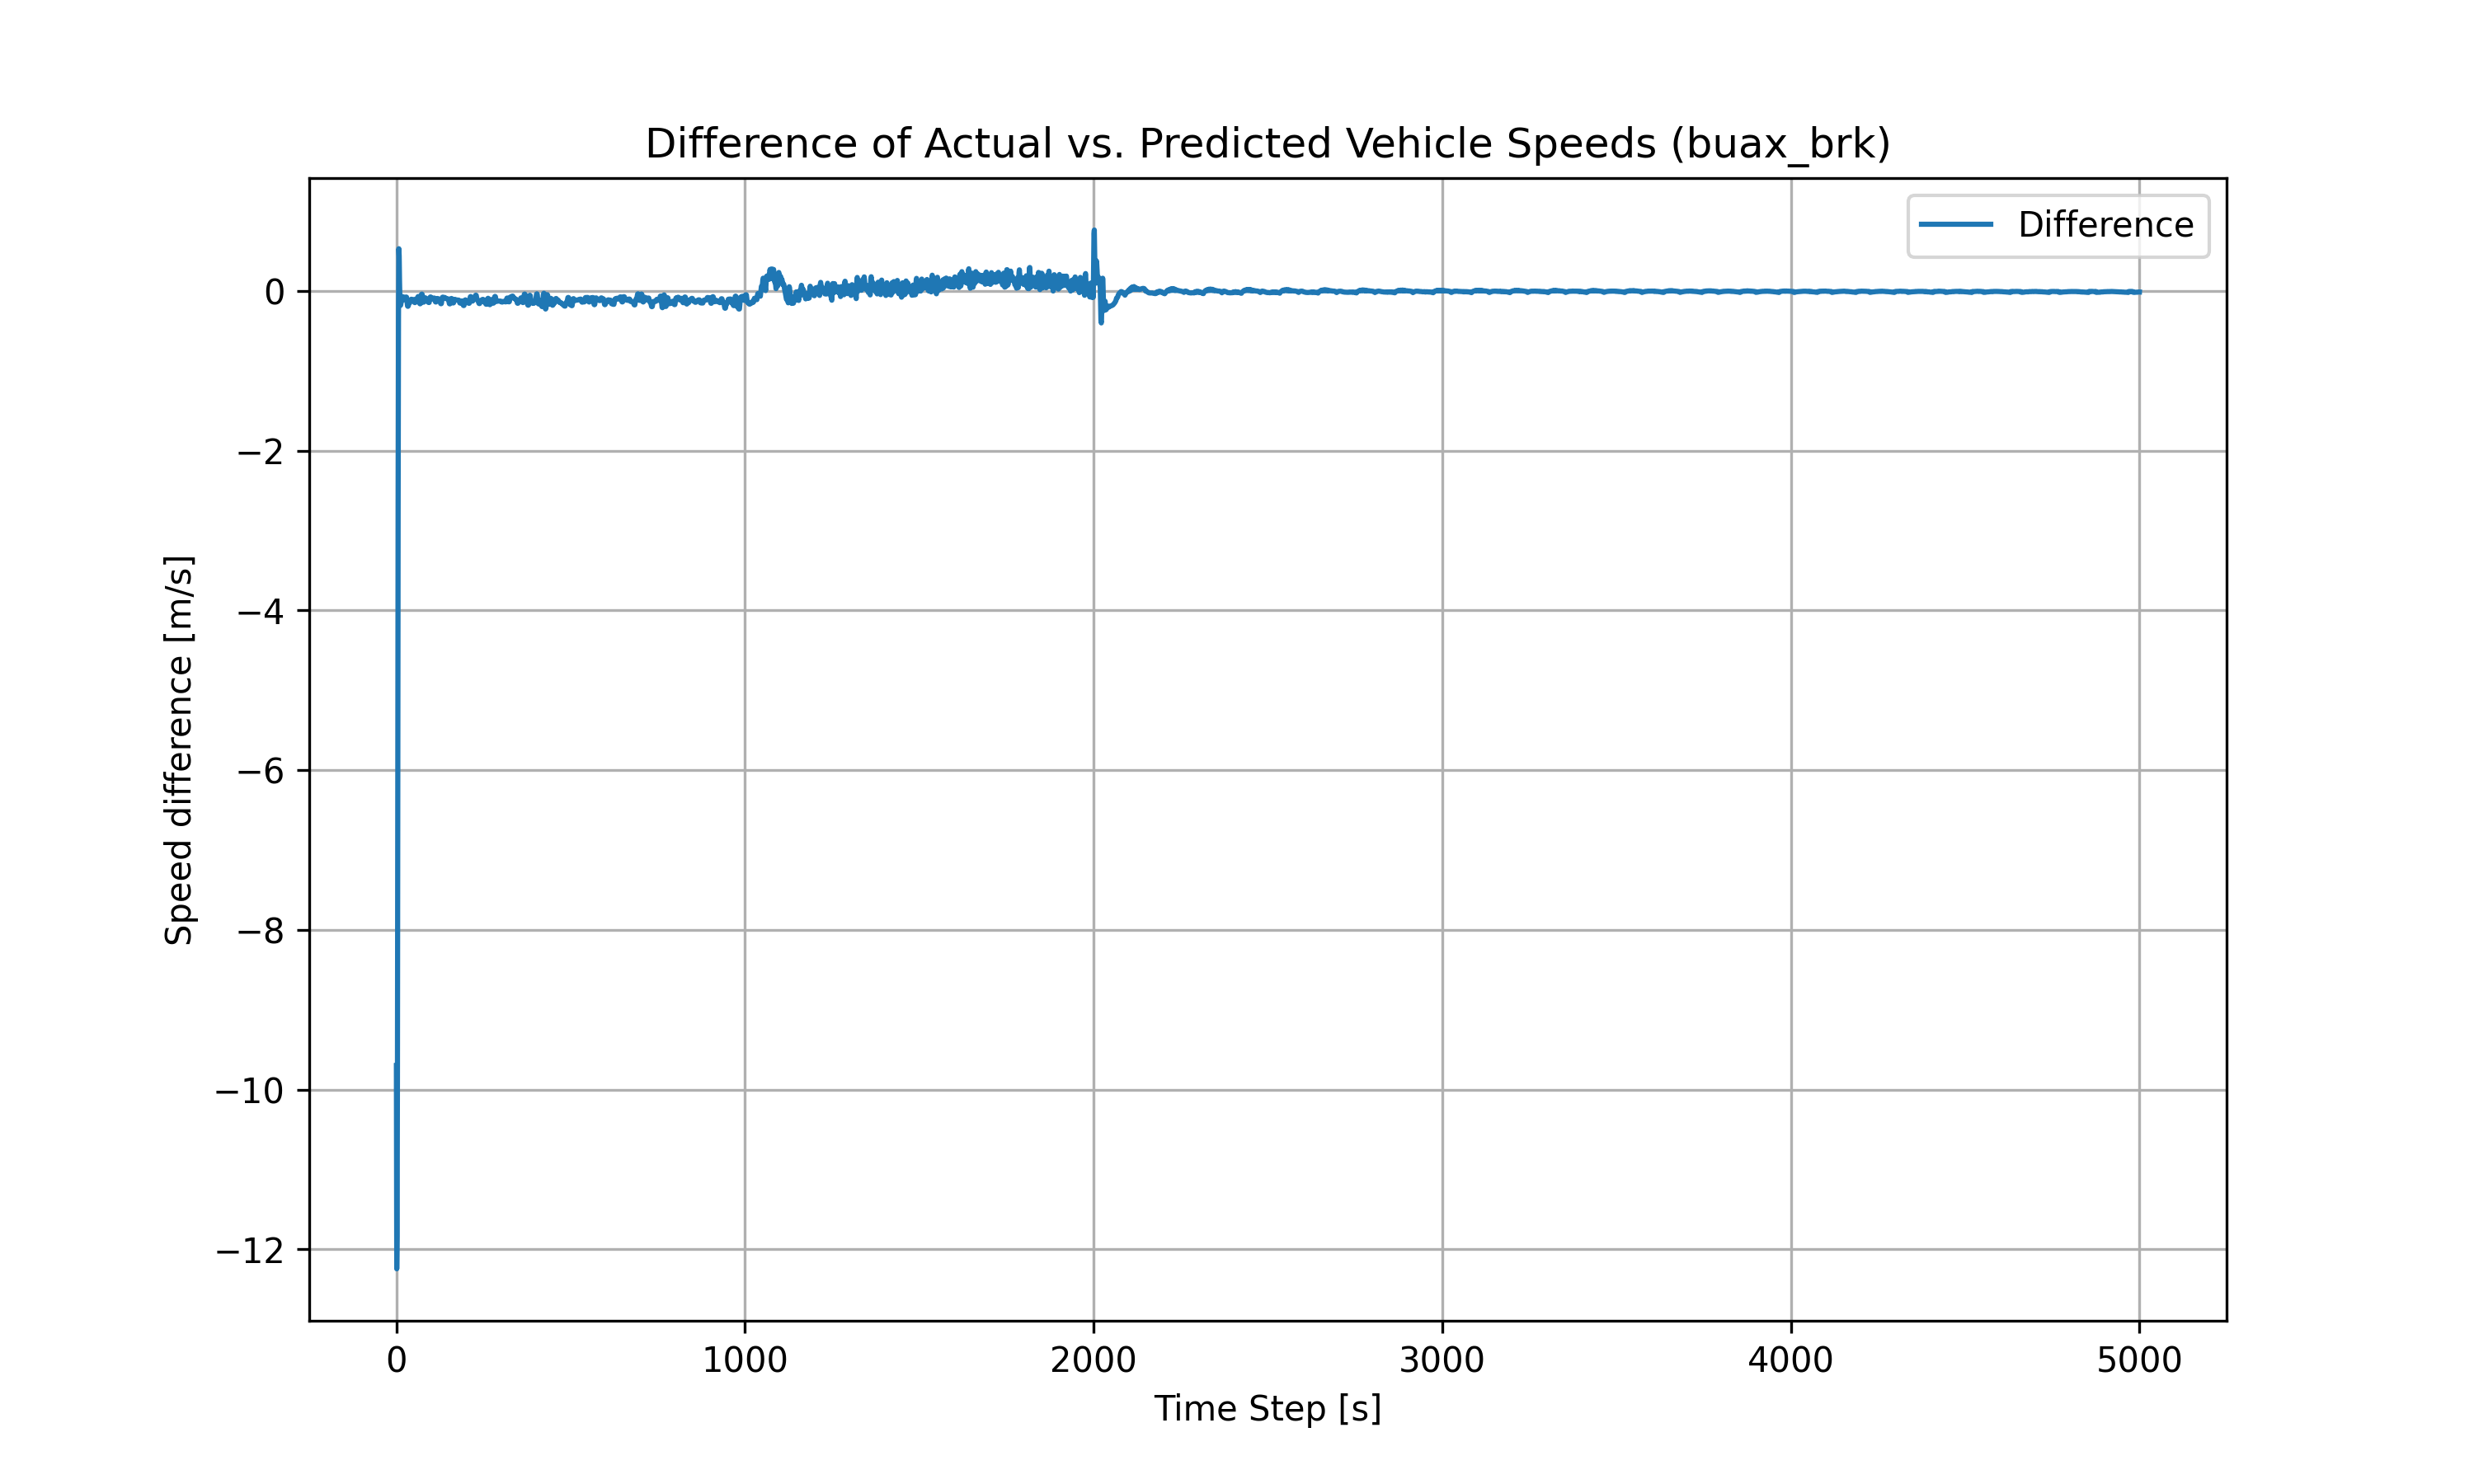
\includegraphics[width=\linewidth]{images/RNN_results/model_0_buax_brk_act_vs_predicted_speed_diff.png}
    \end{subfigure}
    
    \caption{Testing speed estimation with a buay-brk validation dataset}
    \label{fig:rnn_results_buax_brk}
\end{figure}

\begin{figure}[htbp]
    \centering

    % Second row
    \begin{subfigure}{1\textwidth}
        \centering
        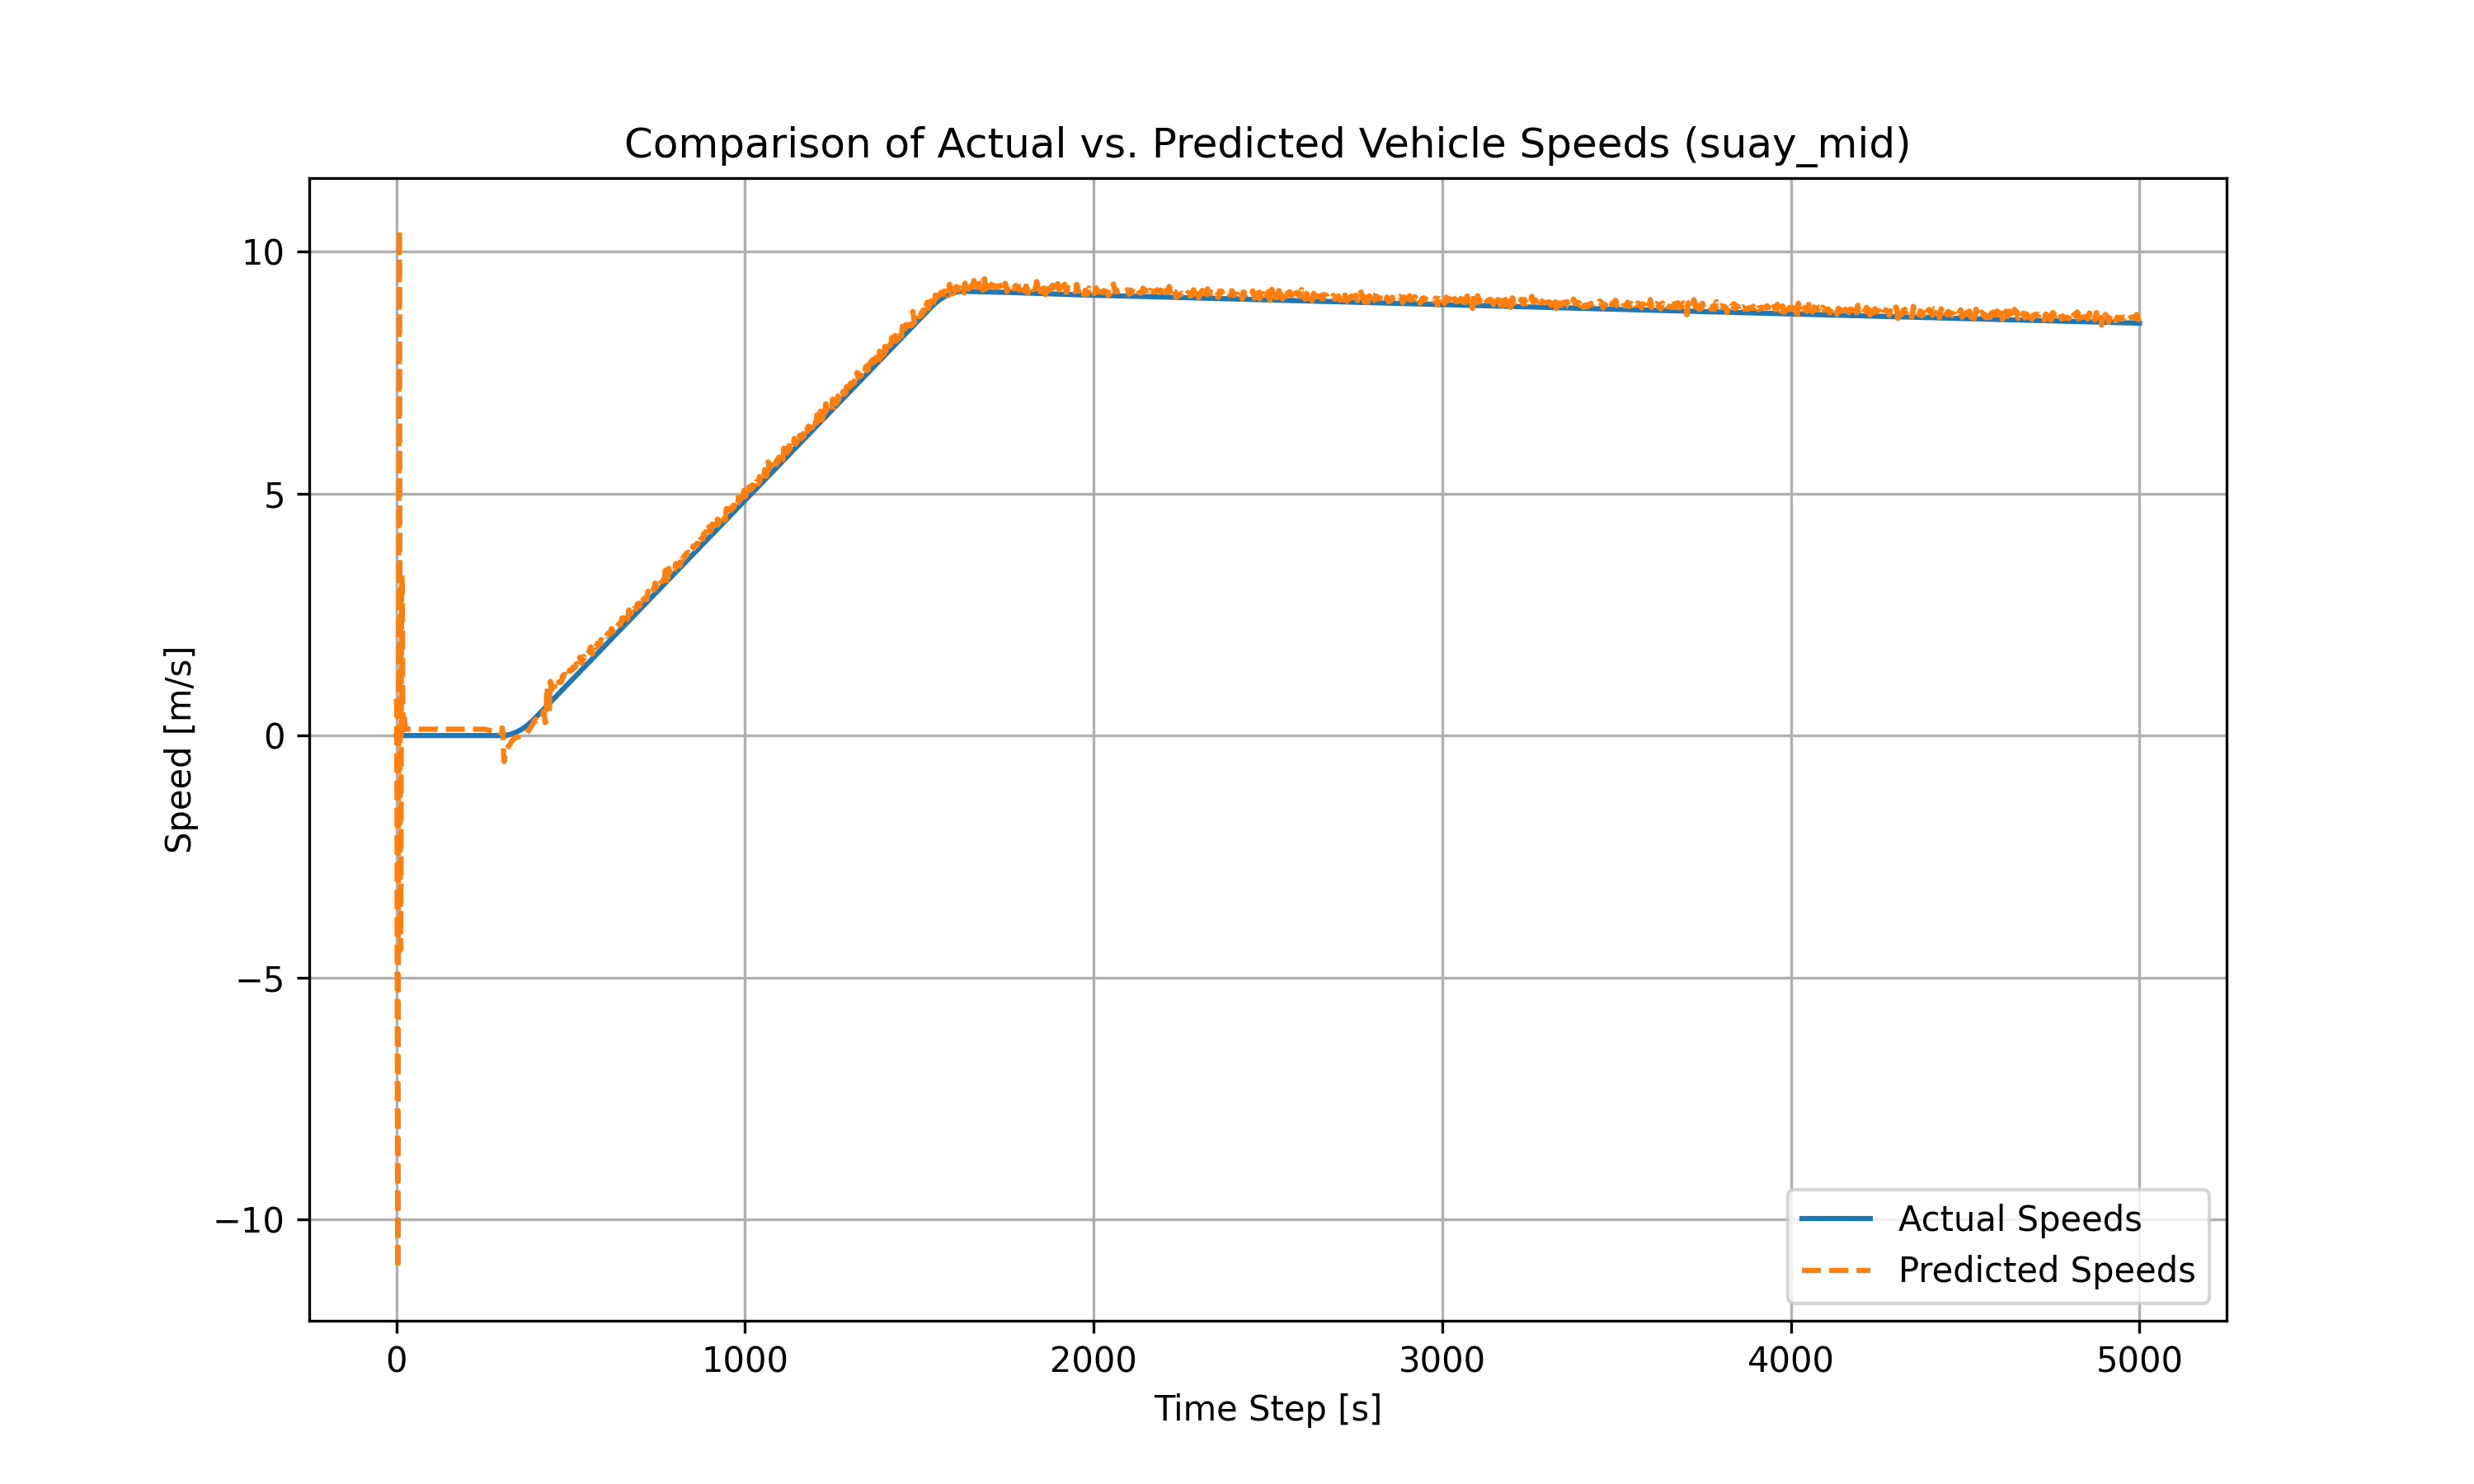
\includegraphics[width=\linewidth]{images/RNN_results/model_0_suay_mid_act_vs_predicted_speed.png}
    \end{subfigure}
    \hfill
    \begin{subfigure}{1\textwidth}
        \centering
        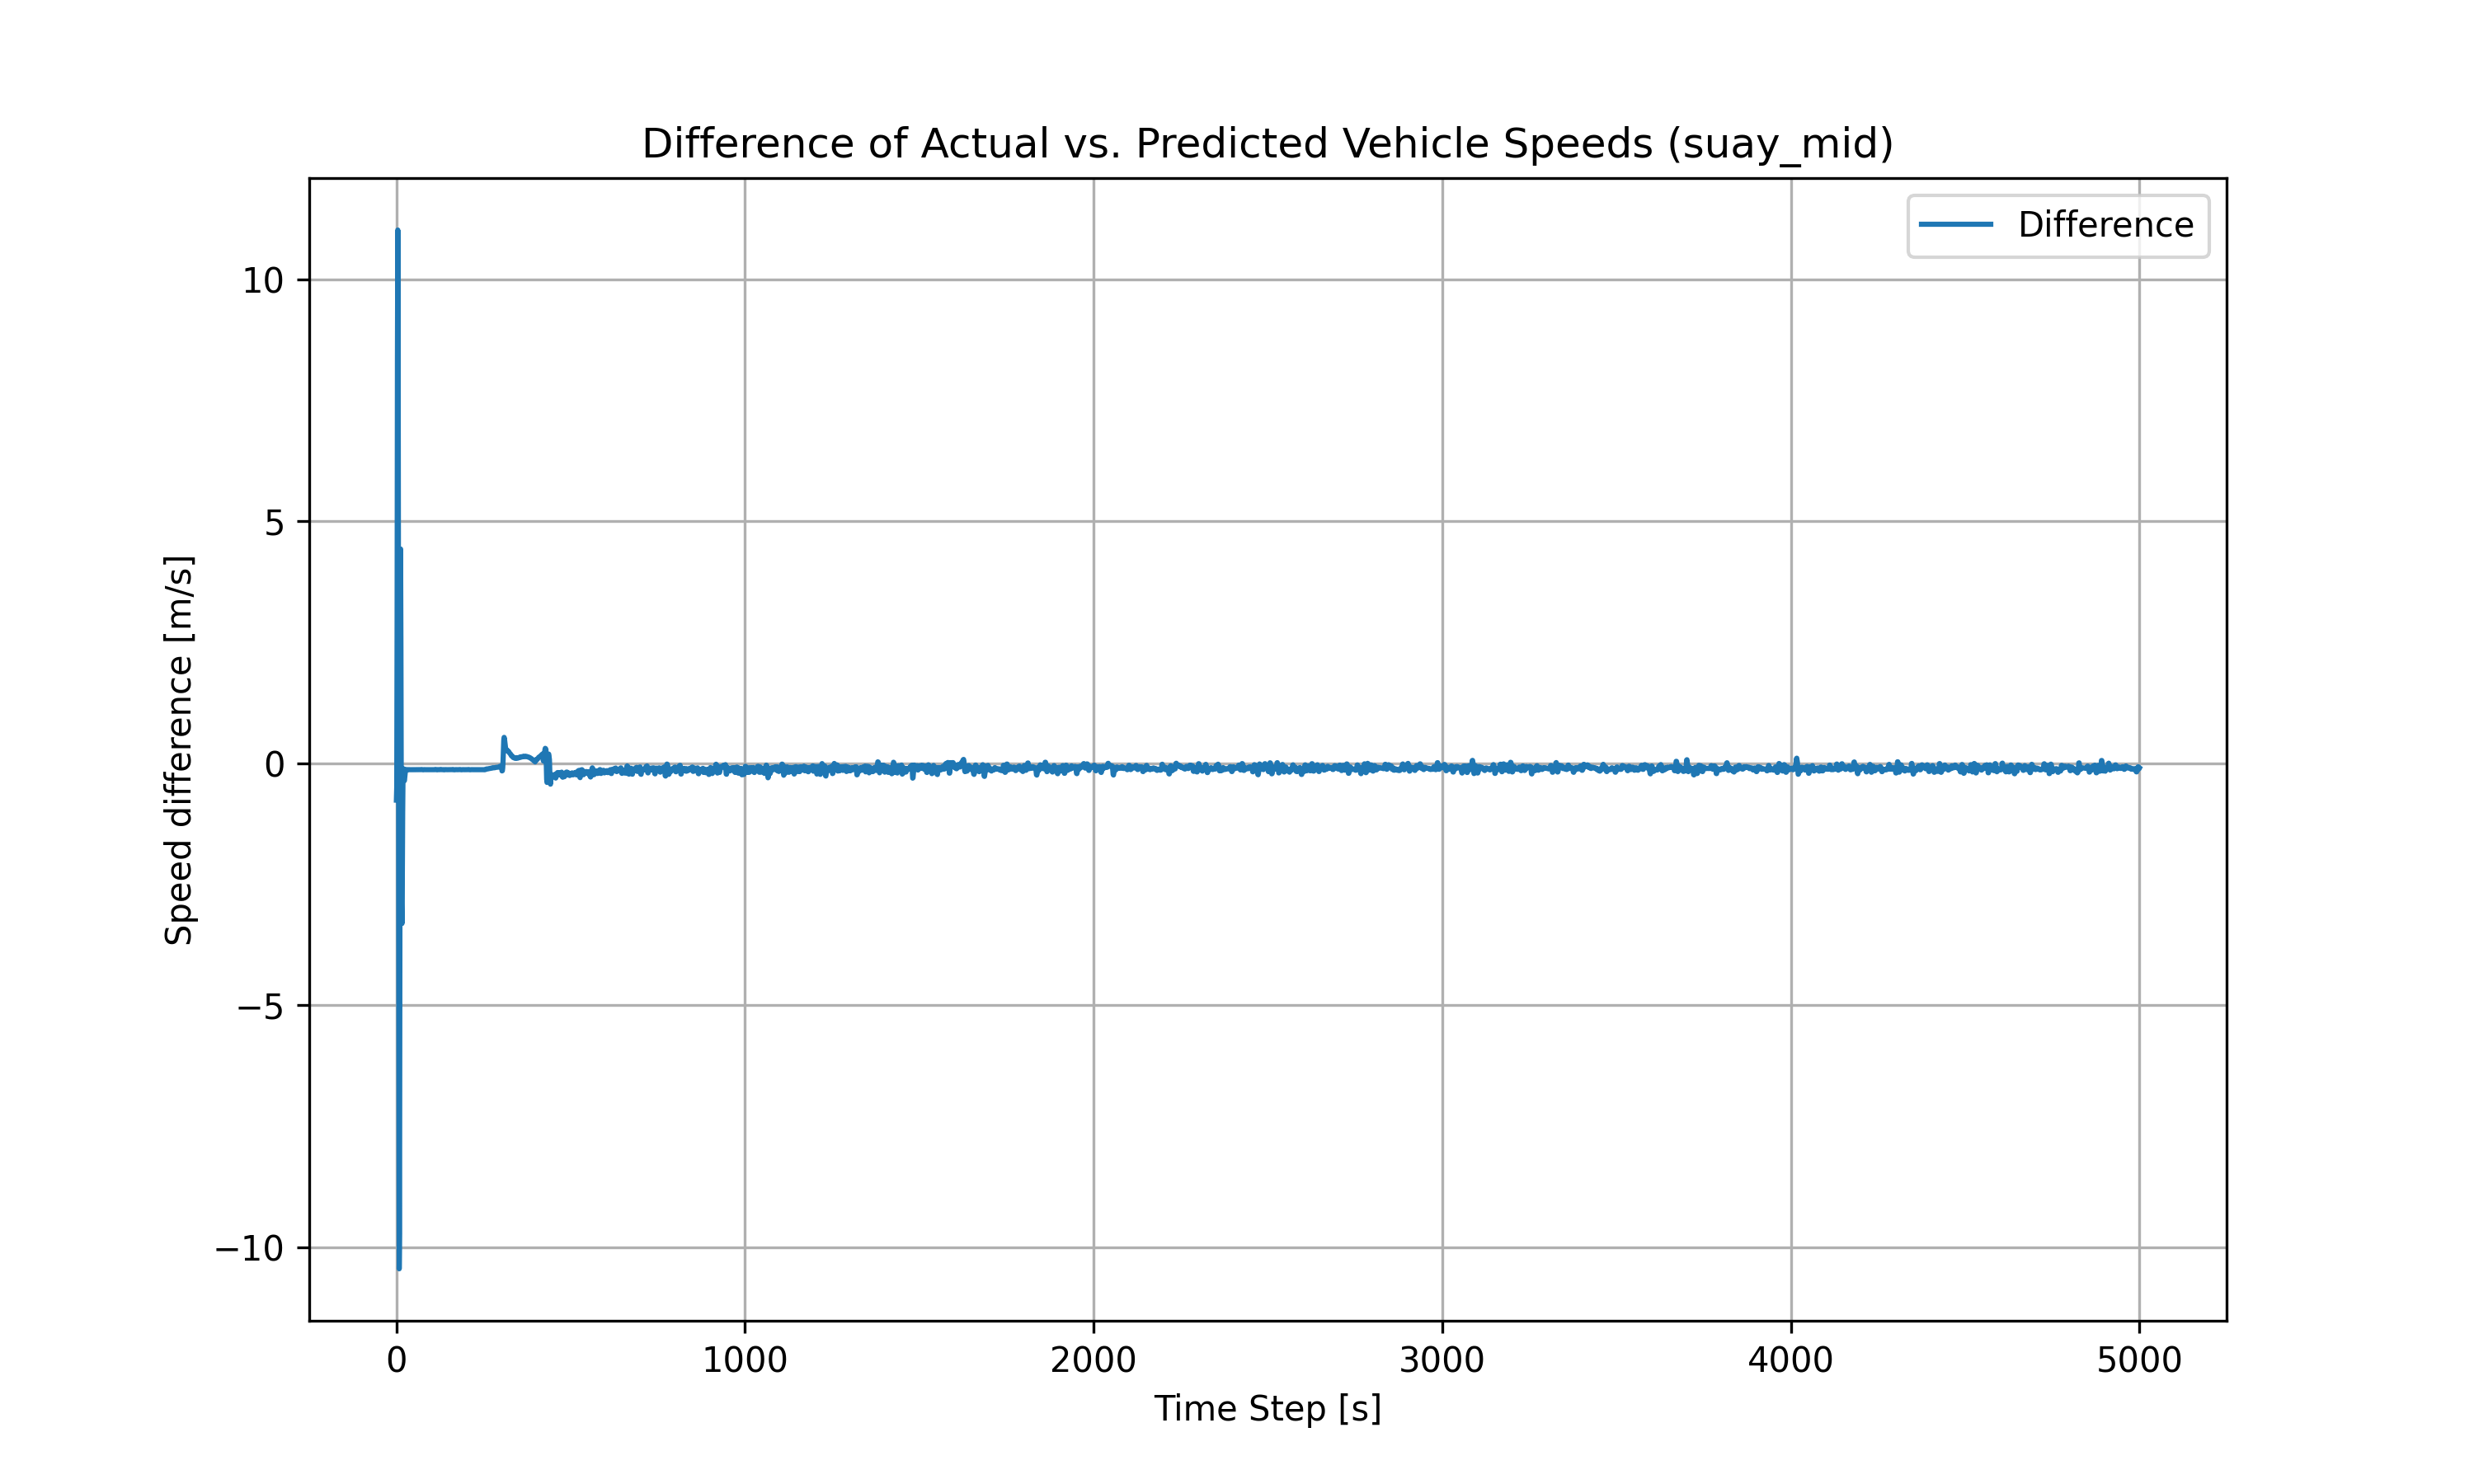
\includegraphics[width=\linewidth]{images/RNN_results/model_0_suay_mid_act_vs_predicted_speed_diff.png}
    \end{subfigure}
    
    \caption{Testing speed estimation with a suay validation dataset}
    \label{fig:rnn_results_suay}
\end{figure}

\begin{figure}[htbp]
    \centering

    % Second row
    \begin{subfigure}{1\textwidth}
        \centering
        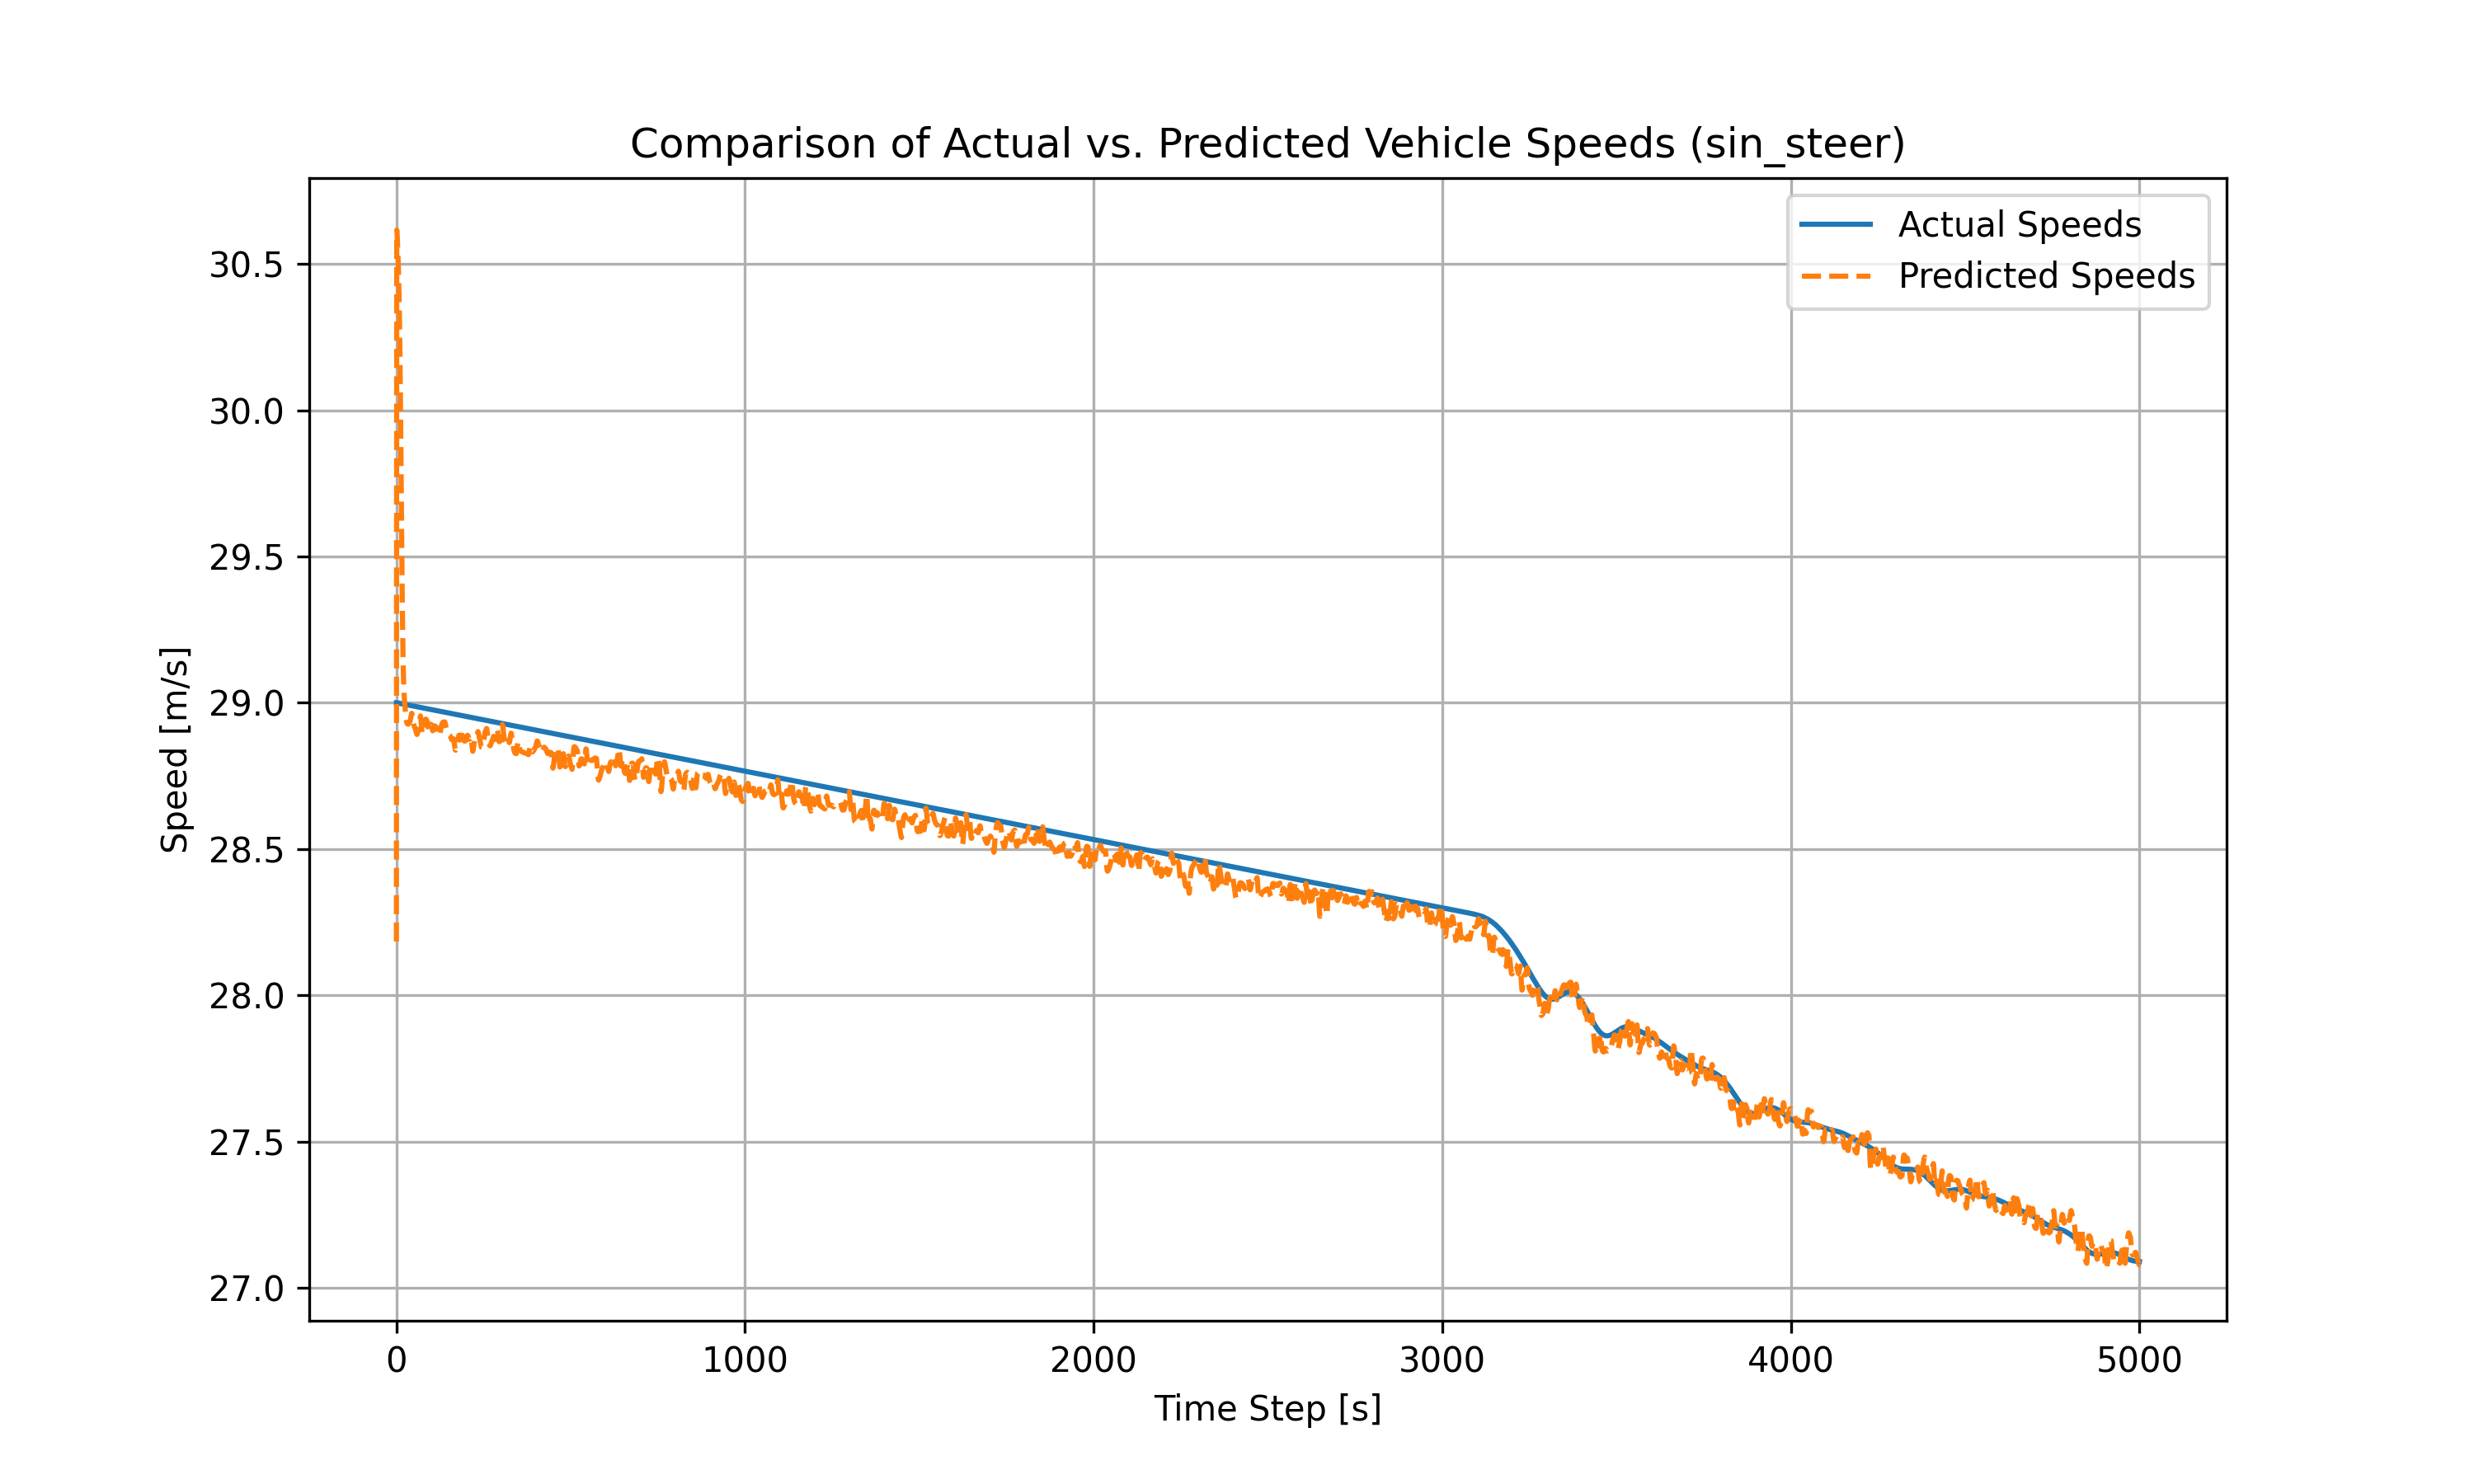
\includegraphics[width=\linewidth]{images/RNN_results/model_0_sin_steer_act_vs_predicted_speed.png}
    \end{subfigure}
    \hfill
    \begin{subfigure}{1\textwidth}
        \centering
        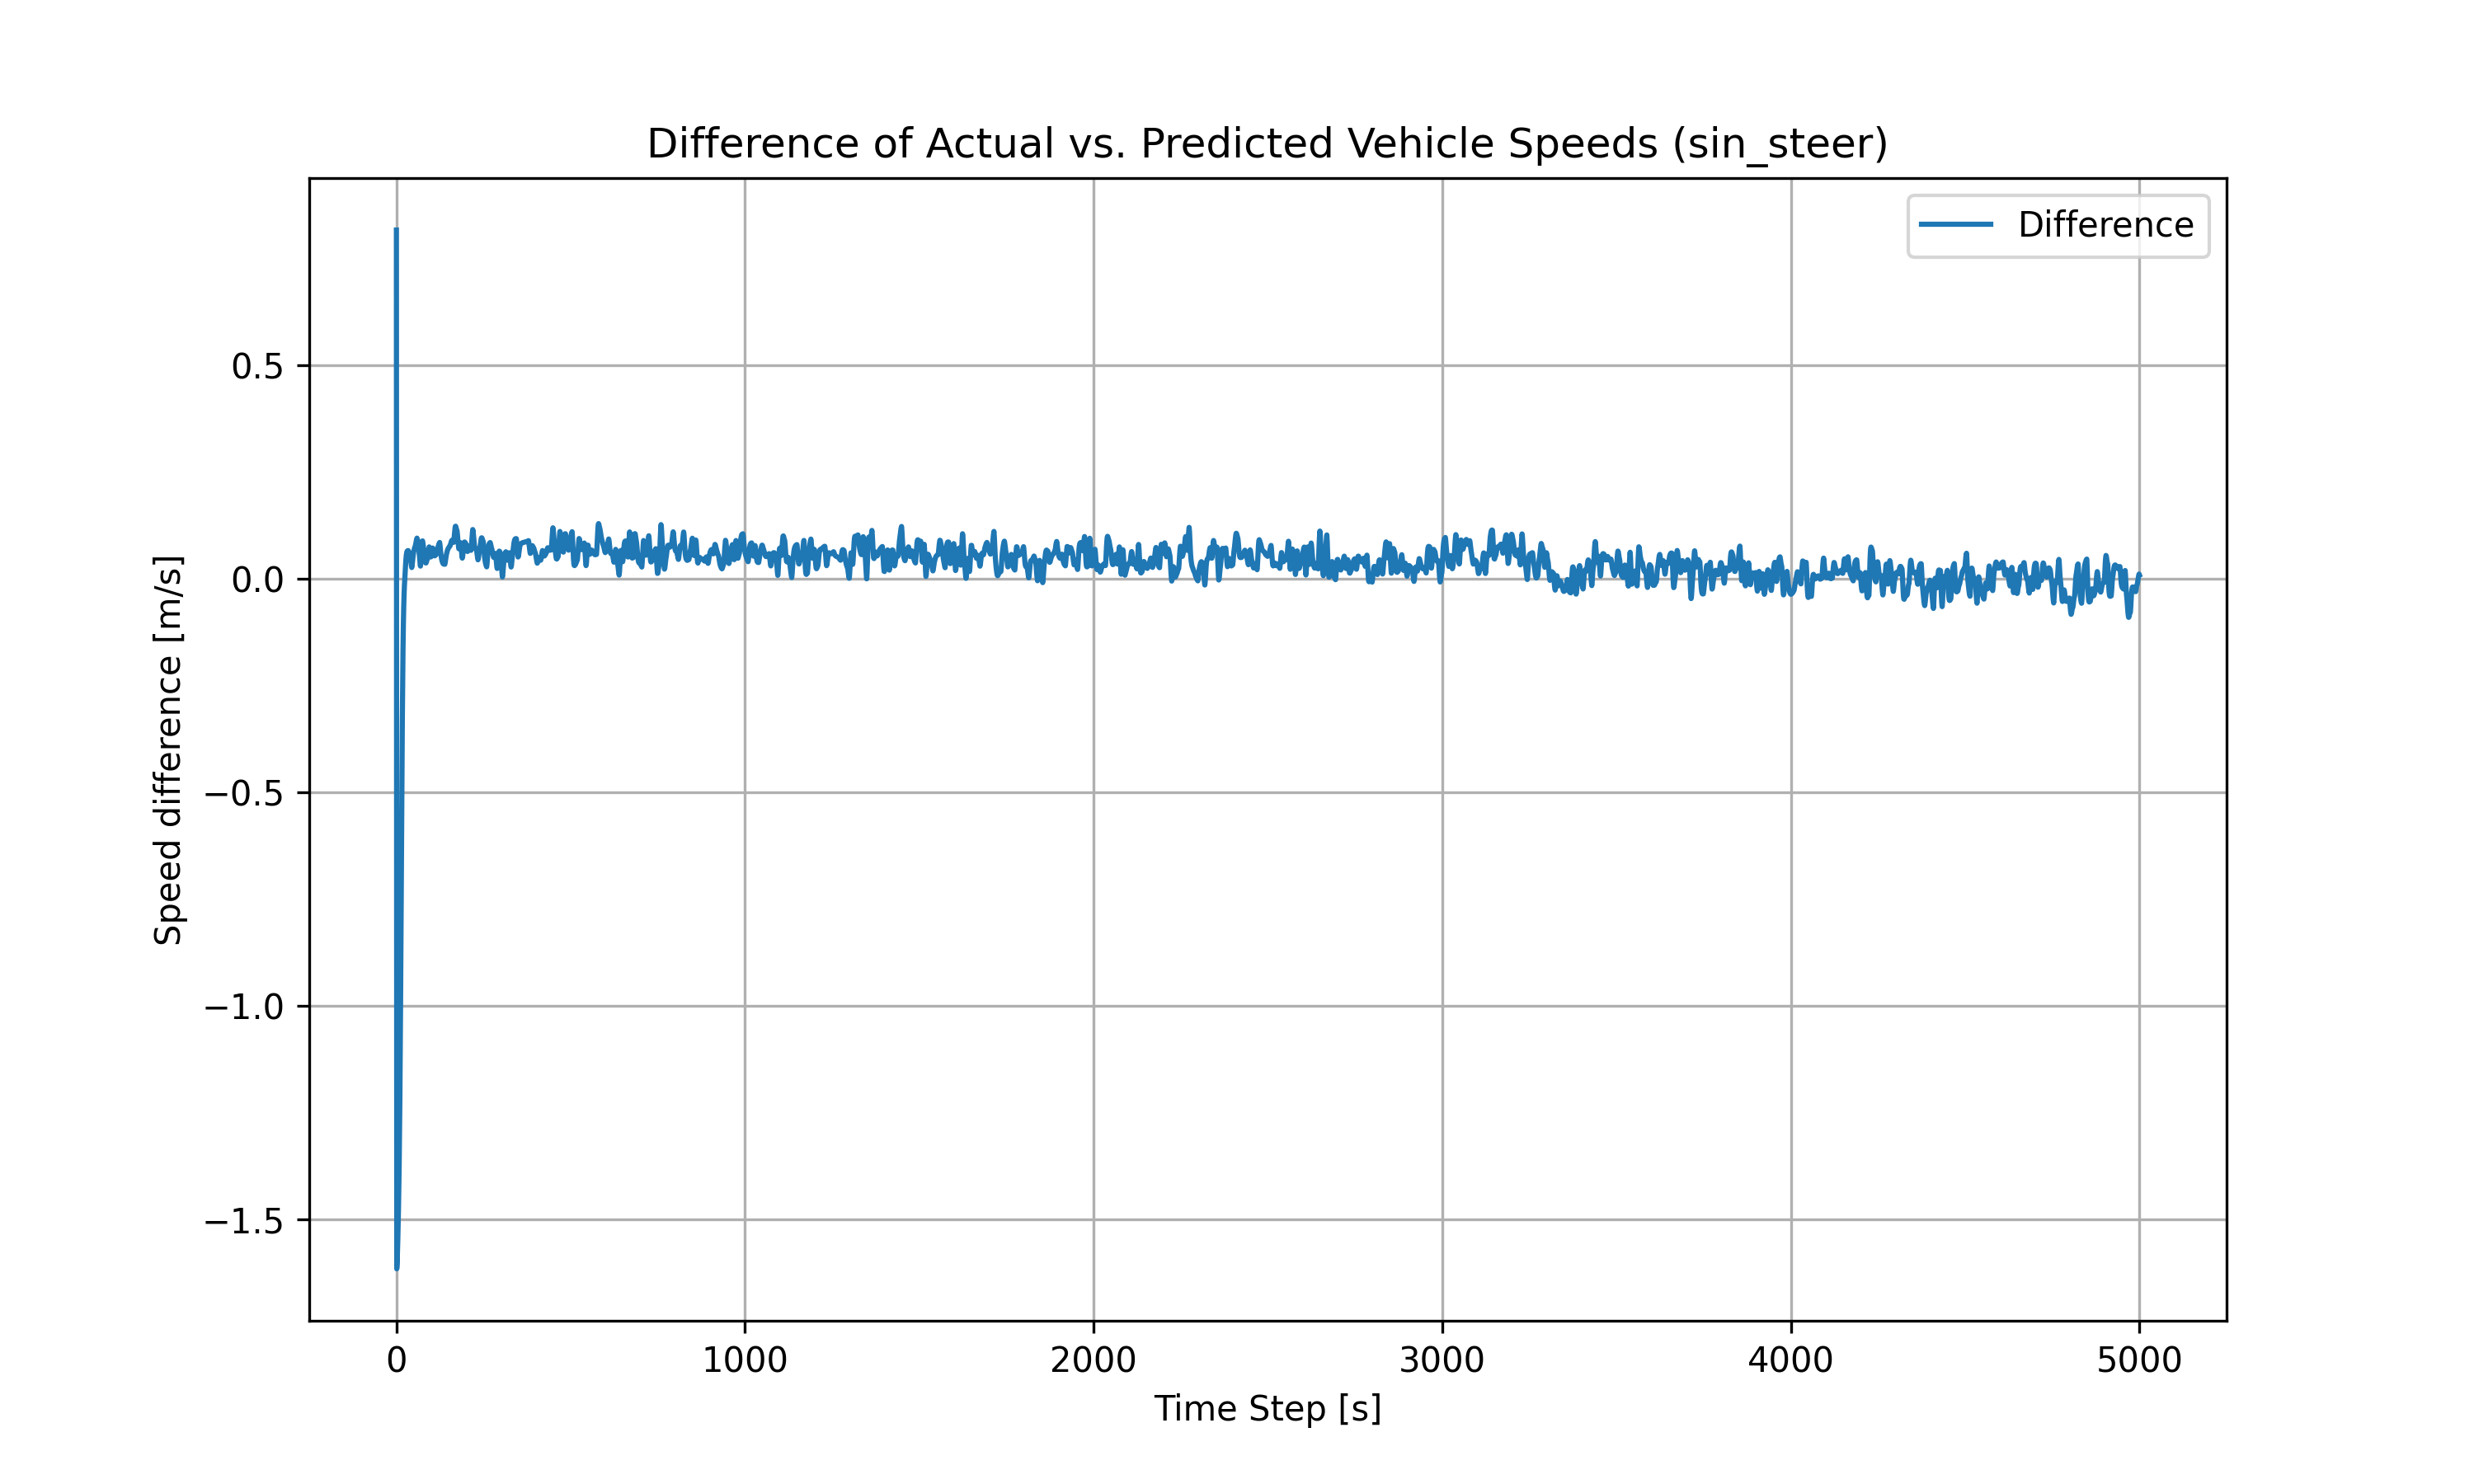
\includegraphics[width=\linewidth]{images/RNN_results/model_0_sin_steer_act_vs_predicted_speed_diff.png}
    \end{subfigure}
    
    \caption{Testing speed estimation with a sin-steer validation dataset}
    \label{fig:rnn_results_sin_steer}
\end{figure}

\begin{figure}[htbp]
    \centering

    % First row
    \begin{subfigure}{1\textwidth}
        \centering
        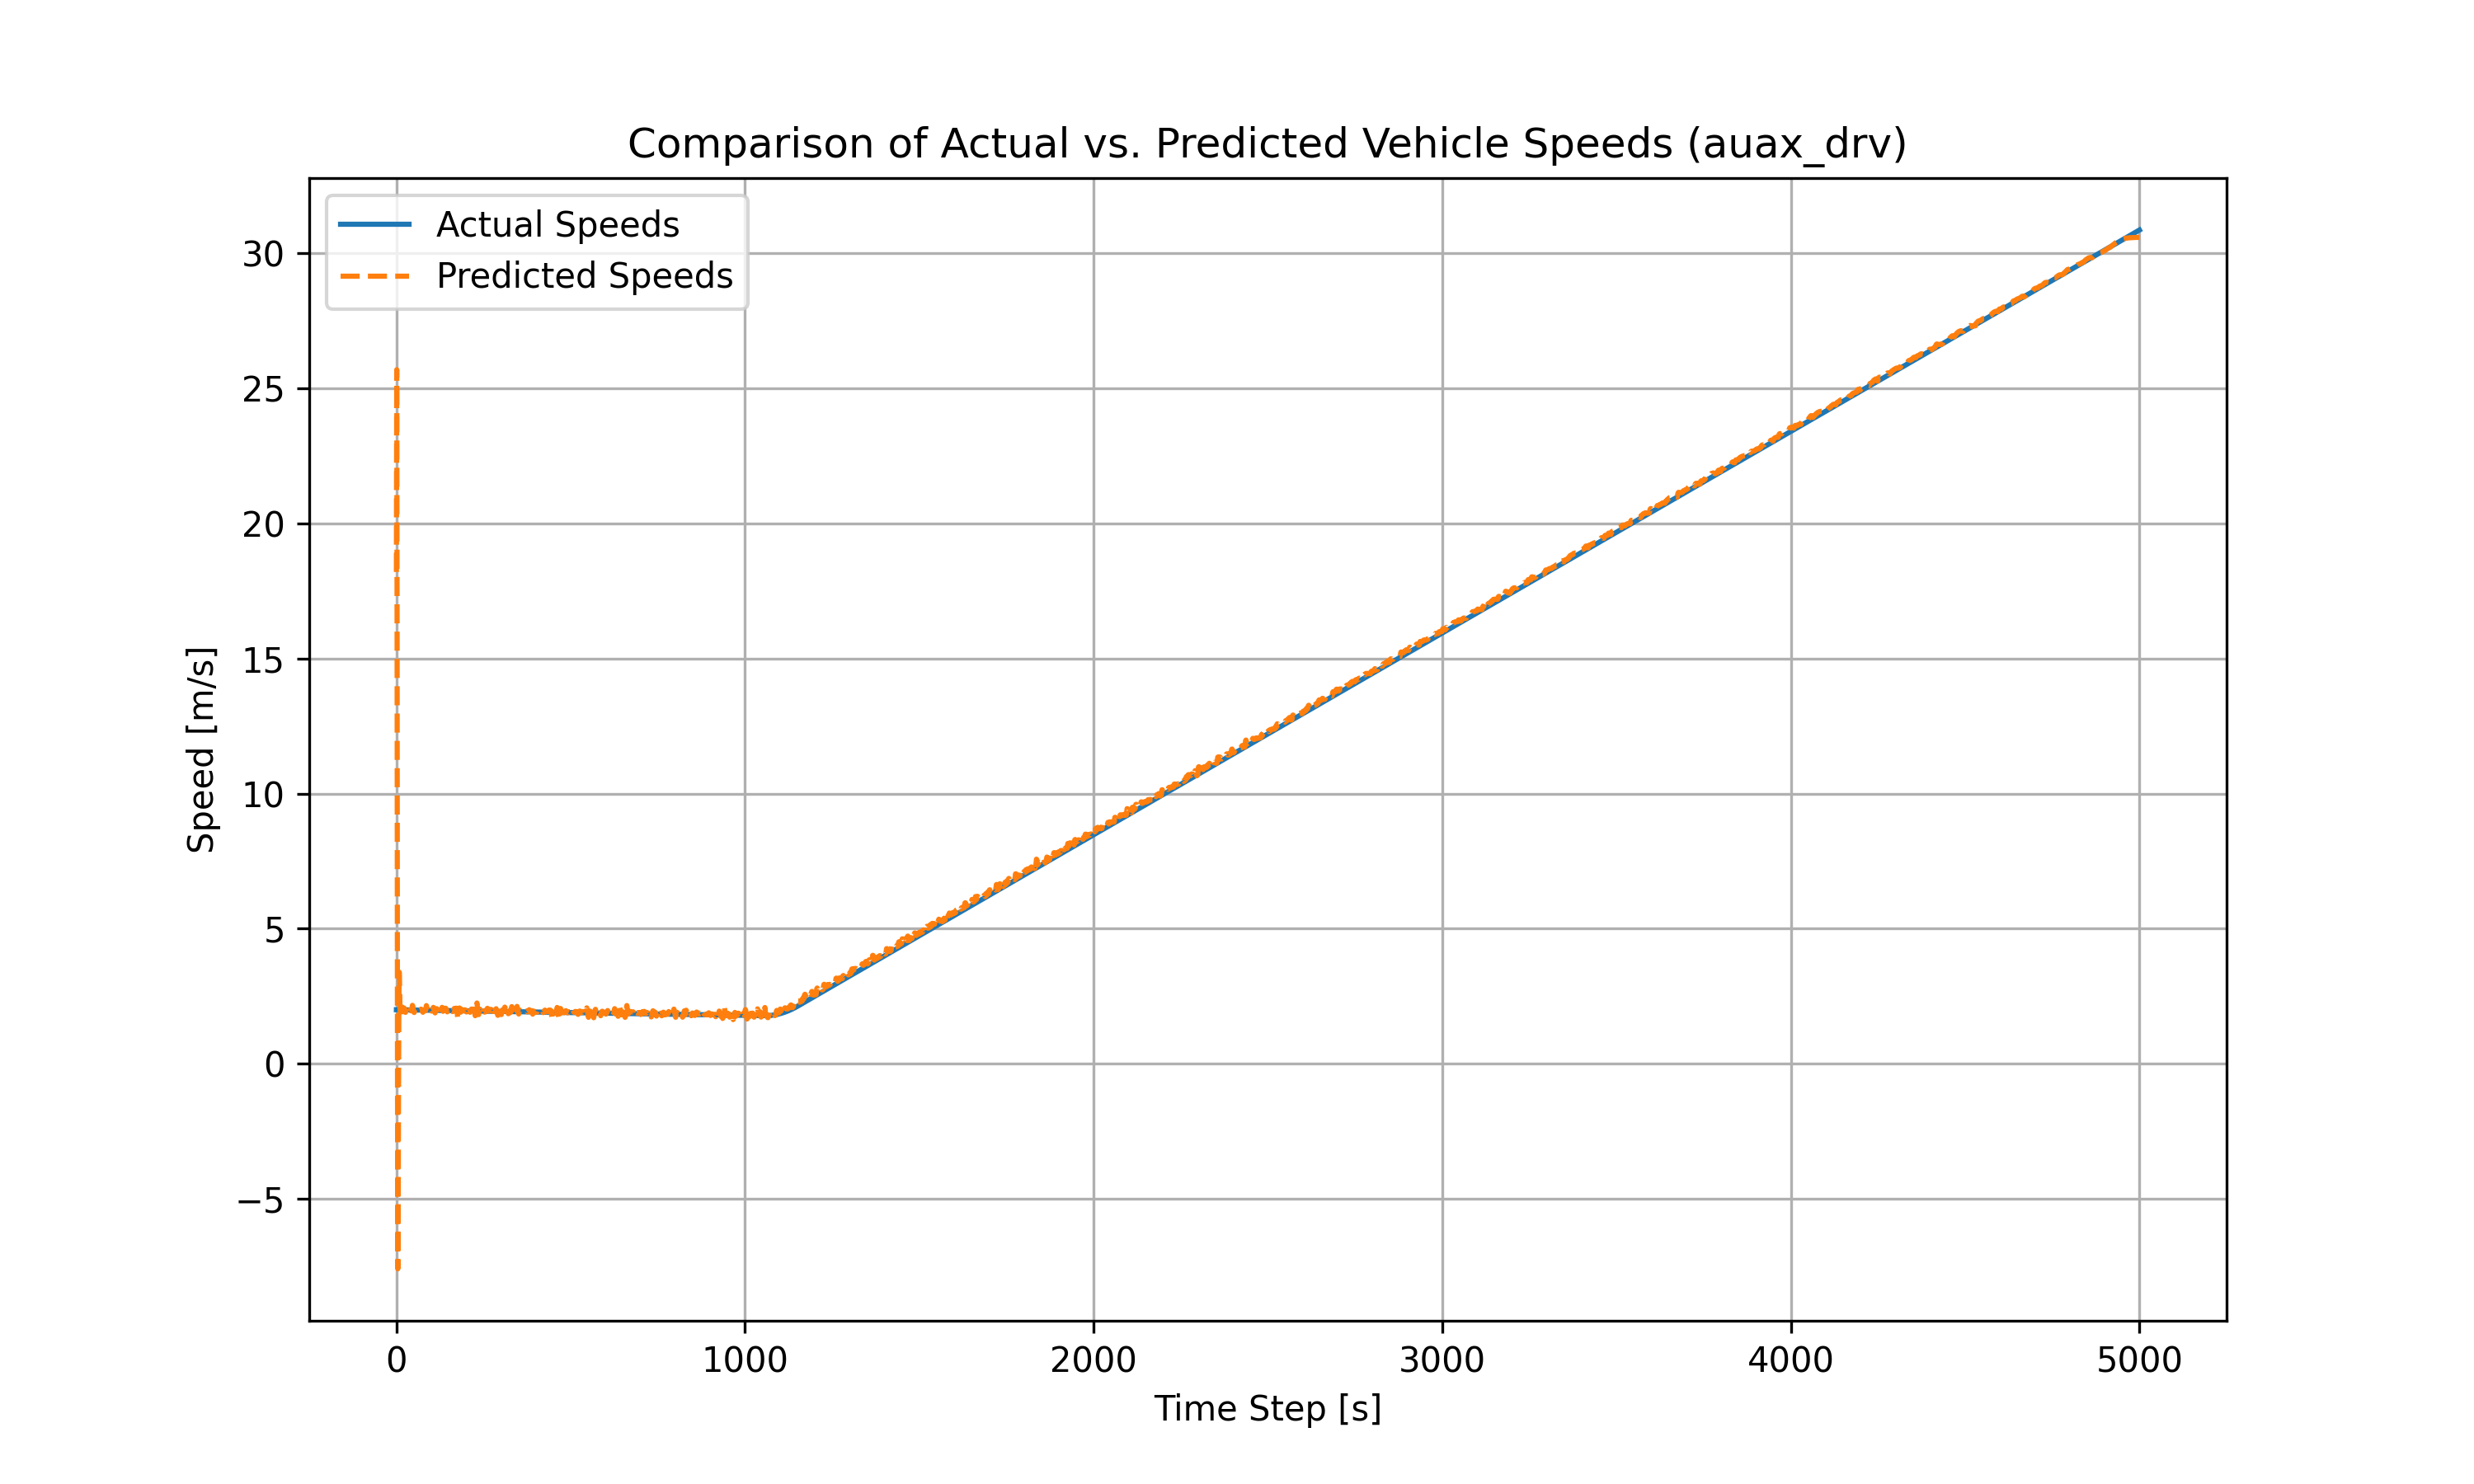
\includegraphics[width=\linewidth]{images/RNN_results/model_0_auax_drv_act_vs_predicted_speed.png}
    \end{subfigure}
    \hfill
    \begin{subfigure}{1\textwidth}
        \centering
        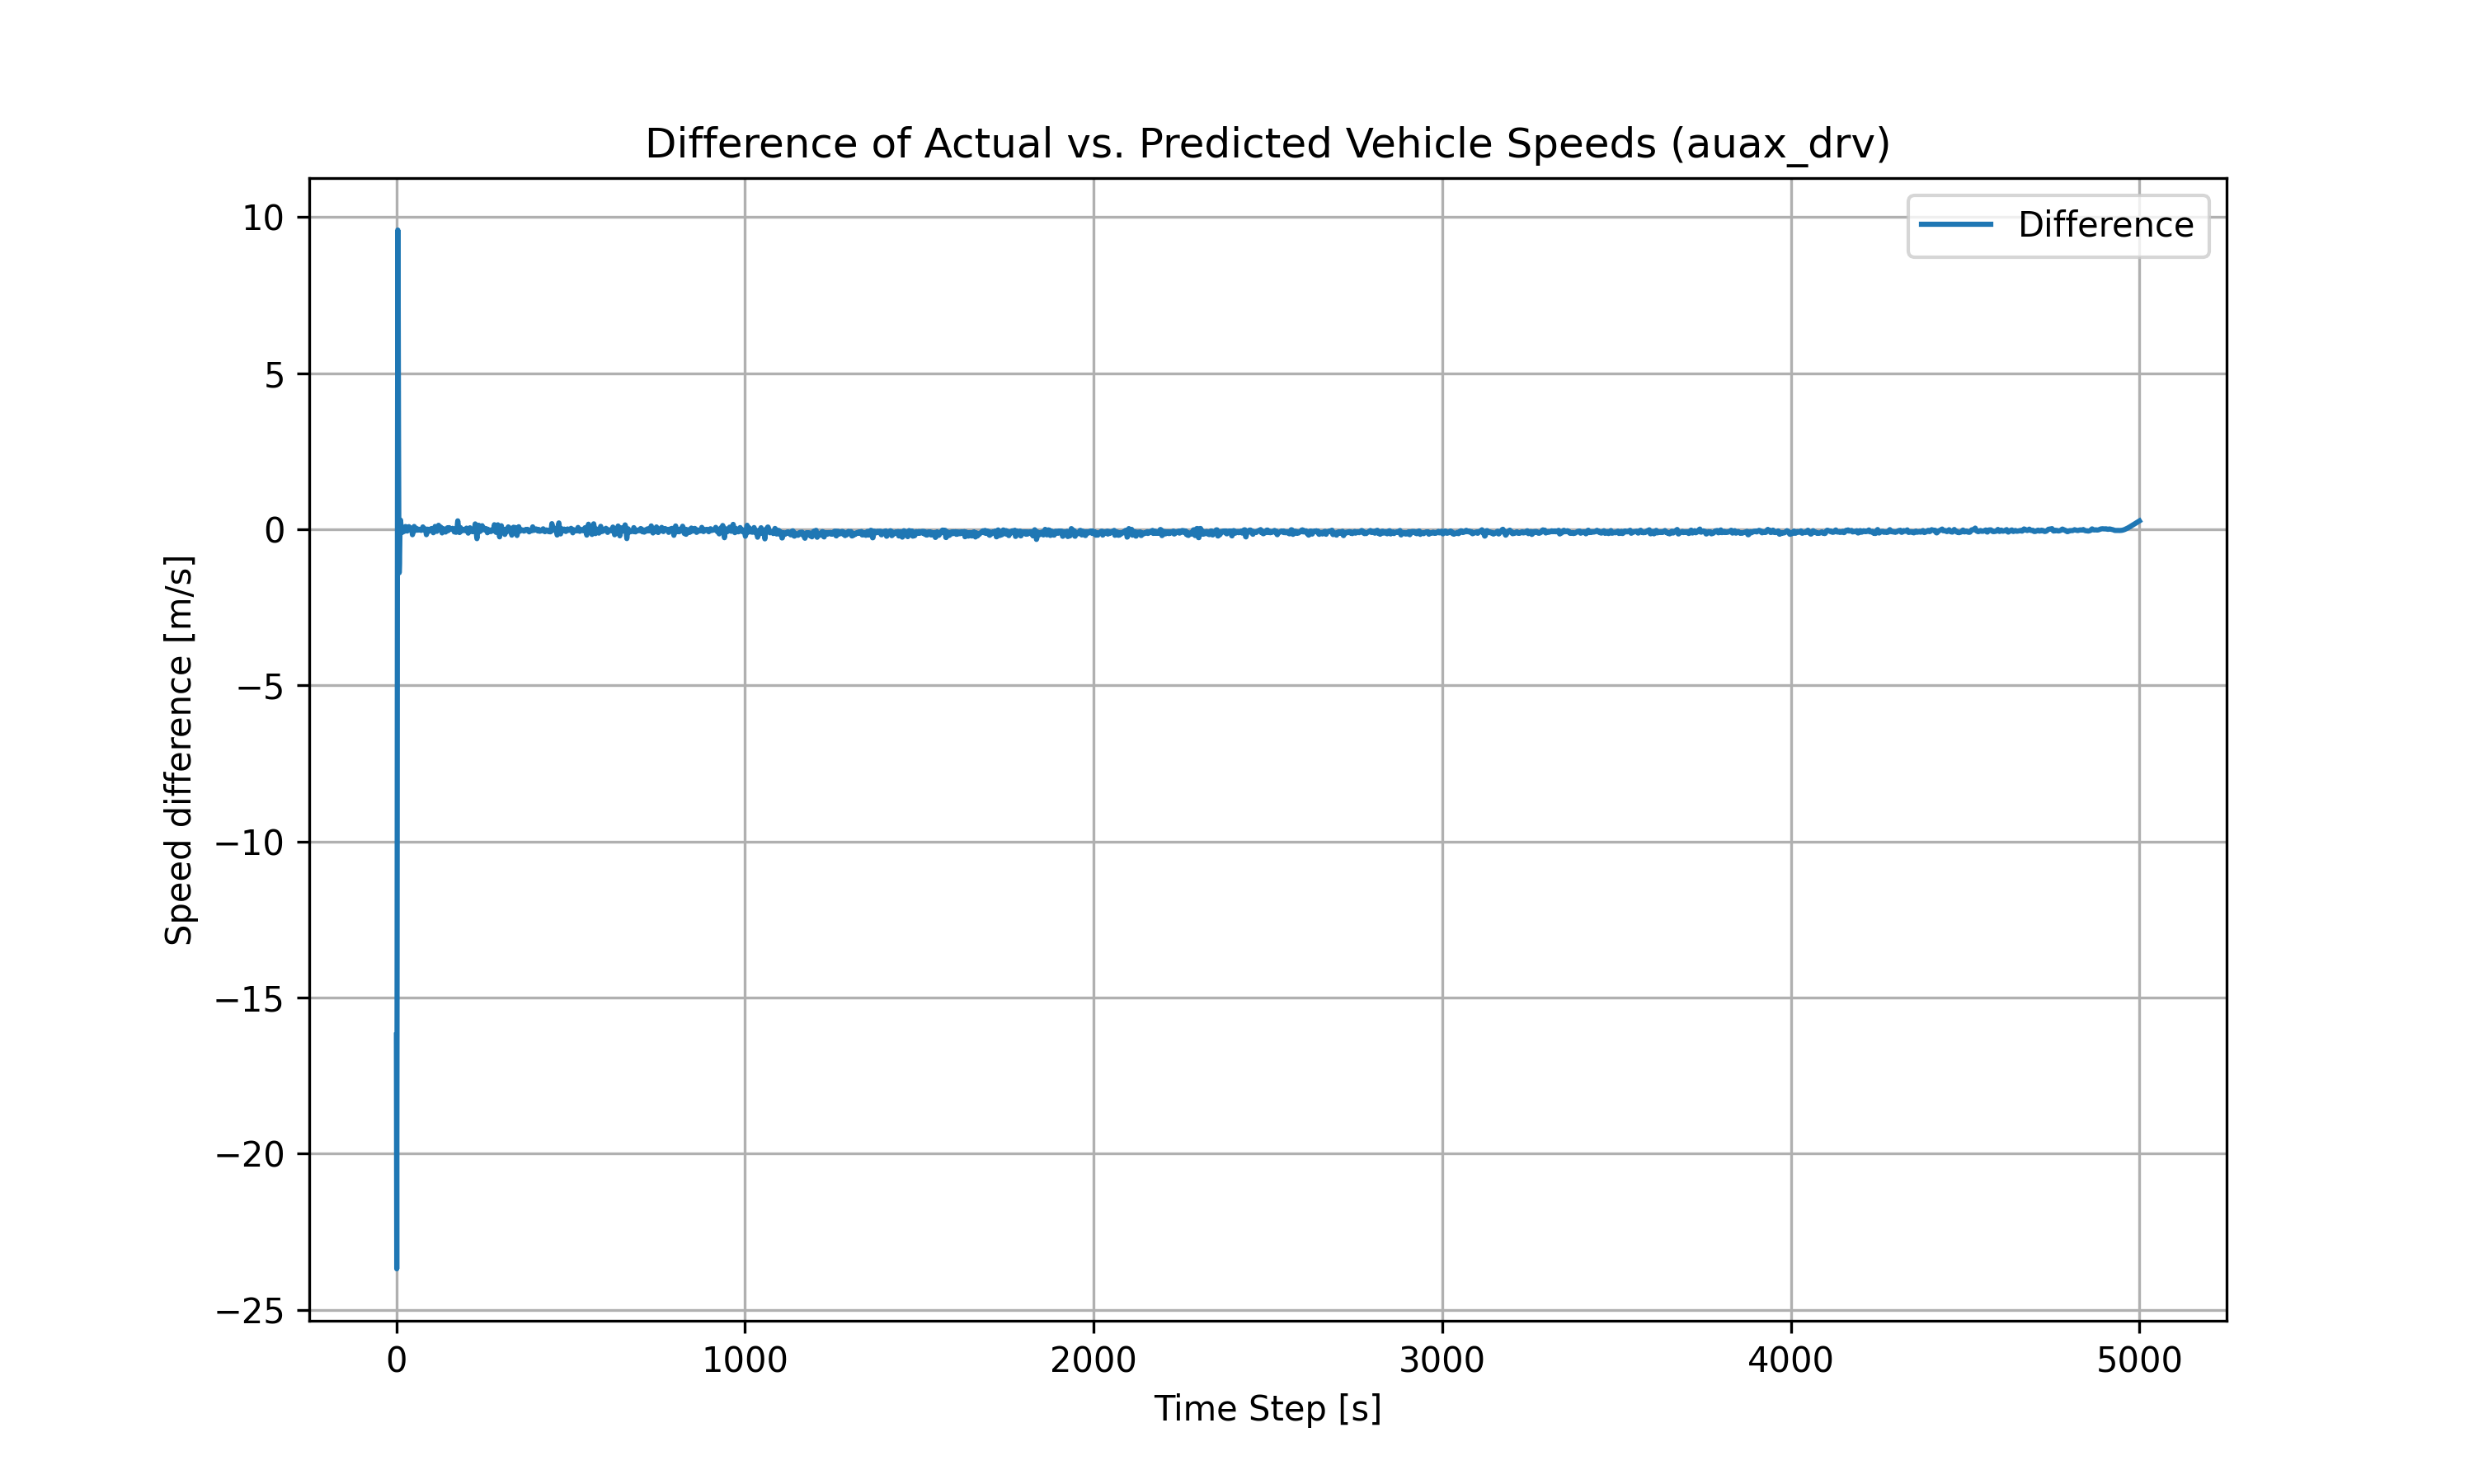
\includegraphics[width=\linewidth]{images/RNN_results/model_0_auax_drv_act_vs_predicted_speed_diff.png}
    \end{subfigure}
    \caption{Testing speed estimation with a auax-drv validation dataset}
    \label{fig:rnn_results_auax_drv}
\end{figure}
\FloatBarrier

It can be seen on the figures that the estimated values for are still not that accurate when replaying the whole simulation. In the beginning, before the number of inputs reach the sequence length, there is a large error due to the missing information as RNNs are trained to estimate based on a sequence. In addition a smoothening algorithm would also improve the quality of the estimation as it is relatively noisy. To further improve the estimator, lateral speed values can be added as an additional output however his will need more resources for training and a larger model to comprehend the new output.  

\section{Scope of further development}

The method that was described above is just the first AI model that can be used. The further development will touch on longitudinal and lateral vehicle speed estimation with LSTM, GRU, Transformers and Temporal convolutional network. In addition, a wider range of test cases will be implemented for training purposes to cover more driving scenarios. To finish it off, some hybrid methods will also be expanded to see and compared with the direct AI estimators. 